\documentclass[11pt, oneside]{book}

\usepackage[spanish, catalan, english]{babel}
\usepackage[utf8]{inputenc}
\usepackage[T1]{fontenc} % from http://www.monperrus.net/martin/producing+searchable+and+copyable+pdf+files+with+accents+using+latex-pdflatex
\usepackage{graphicx}
\usepackage{caption}
\usepackage{subcaption}
\usepackage{multirow}
\usepackage{array}
\usepackage{color, colortbl}
\usepackage{hhline}
\usepackage{eurosym}
\usepackage{parskip}
\usepackage[labelfont=bf]{caption} %labelfont is to make the Figure X.X: in bold
\usepackage[titletoc,toc,page]{appendix}
\usepackage{nameref}
\usepackage[hidelinks]{hyperref}
\usepackage{bookmark}
\usepackage{listings}
\usepackage[algo2e, ruled]{algorithm2e}
\usepackage{pdflscape}
\usepackage{titlesec}
\usepackage{lipsum} %FIXME
%\usepackage[xindy, toc]{glossaries}
\usepackage{glossaries}
\usepackage{multicol}

% Tabular setting
\usepackage[table,xcdraw]{xcolor}
\usepackage{booktabs}
\newcolumntype{M}[1]{>{\centering\arraybackslash}m{#1}}
\newcolumntype{N}{@{}m{0pt}@{}}

% Todo notes
\newcommand\note[1]{\textcolor{red}{#1}}

% Footnote
\usepackage{footnote}
\makesavenoteenv{tabular}
\makesavenoteenv{table}

\usepackage[numbers]{natbib}
\usepackage{amsmath}
\usepackage[toc,page]{appendix}
\usepackage{calligra}

%So that subsubsections appear in the TOC and are numbered
\setcounter{secnumdepth}{3}
\setcounter{tocdepth}{3}

%http://tex.stackexchange.com/questions/11233/distance-between-chapter-title-and-text
\titleformat{\chapter}[hang]{\Huge\bfseries}{\thechapter}{15pt}{\Huge\bfseries}
\titlespacing{\chapter}{0pt}{-50pt}{20pt}

\selectlanguage{english}
\def\Tiny{\fontsize{5pt}{5pt} \selectfont}

\hypersetup
{
    %pdfborder={0 0 0 [0 0]}, % Treu tots bordes dels links
    %kidelinks,               % Treu els bordes dels links
    linkbordercolor={1 1 1},  % Bordes dels links de dins del doc en blanc
    %urlbordercolor={1 1 1},   % Bordes dels links de les url en blanc
    %pdfborder={1 1 0.45},     % Bordes però més prims (0.45)
        % colorlinks=true,          % Coloreja els links (anula linkbordercolor)
        % linkcolor=black,          % Els links en negre com la resta de text
    % Pdf options:
    pdfstartview=FitH,
    pdfauthor={Pablo Pardo Garcia},
    pdfsubject={Master Thesis},
    pdftitle={Automatic Real and Apparent Age Estimation in Still Images},
    pdfkeywords={age estimation, deep learning, biologically inspired features, Msc Thesis},
}

%Commands for references
\newcommand{\myref}[2]{\hyperref[#2]{#1~\ref*{#2}}}
\newcommand{\figref}[1]{\hyperref[#1]{Figure~\ref*{#1}}}
\newcommand{\algref}[1]{\hyperref[#1]{Algorithm~\ref*{#1}}}
\newcommand{\coderef}[1]{\hyperref[#1]{Code~\ref*{#1}}}
\newcommand{\chapterref}[1]{\hyperref[#1]{\ref*{#1}~\nameref*{#1}}}
\newcommand{\annexref}[1]{\hyperref[#1]{Appendix \ref*{#1}~\nameref*{#1}}}

%%%%%%%%%%%%%%%%%%%%%%%%%%%%%%%%%%%%%%%%%%%%%%%%%%%%%%%%%%%%%%%%%%%%%%%
\DontPrintSemicolon
% To make listings and algorithms in the same table of contents.
% from http://tex.stackexchange.com/questions/115023/combine-listoflistings-and-listofalgorithms-into-one-list
\makeatletter
\AtBeginDocument{
    \let\c@algocf\c@lstlisting % Say algorithm2e to use the counter of listings
    \renewcommand{\algocf@list}{lol} % Say algorithm2e to write the material to the listings file lol
    \renewcommand*\l@algocf{\@dottedtocline{1}{1.5em}{2.3em}} % Make the indent of the entries of algorithm and listings equal
}
\makeatother
%%%%%%%%%%%%%%%%%%%%%%%%%%%%%%%%%%%%%%%%%%%%%%%%%%%%%%%%%%%%%%%%%%%%%%%

\lstset{
    breaklines=true,
    captionpos=b,
    basicstyle=\footnotesize \ttfamily,
    frame=single
}
\renewcommand{\lstlistlistingname}{List of Algorithms}


%% Glossary
\makeglossaries
%http://en.wikibooks.org/wiki/LaTeX/Glossary
%https://www.sharelatex.com/learn/Glossaries#Terms


\newacronym{dtw}{DTW}{Dynamic Time Warping}

\newglossaryentry{computer}
{
  name=computer,
  description={is a programmable machine that receives input,
               stores and manipulates data, and provides
               output in a useful format}
}

\newglossaryentry{deictic gesture}
{
    name={deictic gesture},
    description={A gesture that specifies identity or spatial location depending on the context of one or more of the participants in the communication act, which can be accompanied by a deictic utterance such as here, there, this or that},
    plural={deictic gestures}
}

\newglossaryentry{static gesture}
{
    name={static gesture},
    description={A gesture in which the person does not move the whole body or some limbs but rather stays still in a specific position for some short period of time},
    plural={static gestures}
}

\newglossaryentry{dynamic gesture}
{
    name={dynamic gesture},
    description={A gesture which is defined by a movement the person performs with the whole body or a part of it},
    plural={dynamic gestures}
}

%\newglossaryentry{glossaryexample}
%{
%    name={},
%    description={},
%    plural={}
%}

\begin{document}

%Title page
\setcounter{page}{3}
\thispagestyle{empty}
\vspace*{-2cm}

\hbox{

\includegraphics[width=0.7cm]{figures/logoupc.eps}
\includegraphics[width=0.5cm]{figures/logoub.eps}

\includegraphics[width=1cm]{figures/logourv.eps}
\Large \bf Master in Artificial Intelligence (UPC-UB-URV)}
\hrule

%\vfill
%\vfill
\bigskip\bigskip\bigskip

\begin{center}

{\LARGE Master of Science Thesis}

\bigskip\bigskip\bigskip\bigskip\bigskip

\textbf{\huge \bf Automatic Real and Apparent Age Estimation in Still Images}

\bigskip\bigskip\bigskip\bigskip\bigskip

{\LARGE \bf Pablo Pardo Garcia}

\end{center}
\vspace*{3cm}

\begin{center}
{\large Supervisor:}
\end{center}

\medskip %\medskip\smallskip

{\Large\bf Sergio Escalera Guerrero}

\medskip %\medskip

{Dept. Matemàtica Aplicada i Anàlisi, University of Barcelona}

\medskip

%{\Large University of Barcelona}

%{\Large Master in Artificial Intelligence}

\bigskip %\bigskip\bigskip

\begin{center}
{\large Co-supervisors:}
\end{center}
%\begin{multicols}{2}
	
\medskip %\medskip\smallskip

{\Large\bf Marc Oliu Simón}

\medskip %\medskip

{Dept. Matemàtica Aplicada i Anàlisi, University of Barcelona}

%{\Large University of Barcelona}

\medskip %\medskip\smallskip\medskip

{\Large\bf Isabelle Guyon}

\medskip %\medskip

{President at ChaLearn and Clopinet, Berkeley, California}


%\end{multicols}

\medskip\medskip\medskip\medskip\medskip

% This has obviously to be changed
\begin{center}
{\Large Barcelona, 24th April 2015}
\end{center}

%\clearpage

%\thispagestyle{empty}
%\ 
%\clearpage


\chapter*{} % empty chapter to have a blank page after the title
\thispagestyle{empty}

\thispagestyle{empty}
\chapter*{Acknowledgements}
\thispagestyle{empty}

I would like to thank my supervisor Sergio Escalera for supporting and believing in me. This work would have been much harder without the incredible help of Marc Oliu and Xavi Baró who guide me though the deep learning and web developer world.

I also want to thank Google, Microsoft and California Naturel for sponsoring the international challenge we are organizing out of this project. Also thank AgeGuess research group for their collaboration with our project.

And last but not least, this work would not have been the same without my gang, you are a source of energy and inspiration. Hope this still the same in our new and soon coming adventures.

\pagenumbering{arabic}
\setcounter{page}{0}
\clearpage

%Table of contents
\newpage
\pagenumbering{roman} % Roman numerals
\chapter*{Abstract}


\selectlanguage{catalan}
\chapter*{Resum {\small (Catalan)}}

\selectlanguage{spanish}
\chapter*{Resumen {\small (Spanish)}}


\selectlanguage{english} \selectlanguage{english}
\tableofcontents
\listoftables
\listoffigures

\newpage
\pagenumbering{arabic} % Normal numerals

%Document
\chapter{Introduction} \label{chap:introduction}

Computer Vision is a very important field in Artificial Intelligence that exists since the 1960s when digital image processing by computers became possible. Since the beginning of artificial vision, facial analysis has been a major interest in the research community (not just in Computer Vision but in other scientific areas such as biology \cite{bhl24064}, psychology \cite{ekm02}, neuroscience \cite{freiwald2009face} and sociology \cite{kemper1978social}) because its difficulty and its applications. Some of its applications include automatic detection of facial expressions \cite{cohen2003facial}, face detection \cite{hsu2002face}, face recognition \cite{wright2009robust} \cite{taigman2014deepface} and automatic estimation of age \cite{4359348}, gender \cite{alexandre2010gender} and ethnicity \cite{hosoi2004ethnicity}.

Age estimation is a field within the facial analysis area in Computer Vision that tackles the problem of automatically predicting the age of people from visual data (still images, video data, depth maps, etc.). One of the main issues that the age estimation problem has is that there are many factors that influence human perception of age, some factors affect the aging of a person \cite{shephard1997aging}, such as smoking, drinking alcohol, doing sports, alimentation, etc. and others affect the face appealing such as scars, plastic surgery, make-up, facial hair, etc.

Some definitions should be established beforehand regarding the concept of human age:
\begin{itemize}
	\item \textit{Real age}: The actual age (time elapsed since the person was born).
	\item \textit{Apparent age}: Perceived age from humans from the visual appearance. 
	\item \textit{Estimated age}: The predicted age by a machine from the visual appearance.
\end{itemize}

\section{Goals}
This work aims to study the differences (if any) of automatic age estimation from real age labels and apparent age labels. Given that does not exist any face image dataset with this two label annotations, a database with such requisites has been created. In order to do so, a web-based application was developed using the \textit{Facebook API} to facilitate a collaborative and competitive collection of face images.

As a consequence of this work, the first database in the literature containing real age and apparent age annotations for the face images was created and analysed. This database will allow researchers to tackle a different and new sub-problem of age estimation, \textit{Apparent Age Estimation}. The most important methods in the state of the art are evaluated over our proposed database in this work.

In \textit{Real Age Estimation} other external factors such as time evolution, habits and surgeries have to be taken into account. However \textit{Apparent Age Estimation} is based purely in the perception field.


\section{Age Challenge}

Given the innovative aspect of the database, the HuPBA (Human Pose and Behaviour Analysis) research group\footnote{Human Pose and Behaviour Analysis research group\\ \url{http://www.maia.ub.es/~sergio/soluciones2_008.htm}} together with the company ChaLearn\footnote{ChaLearn: Challenges in Machine Learning: \url{http://www.chalearn.org/}} are going to prepare an international challenge competition later this year and present the results in a workshop organized by the team in the ICCV conference 2015 edition (under revision) within the ChaLearn Looking at People series \cite{LaP} \cite{SergioEscalera2014} \cite{Escalera:2013:MGR:2522848.2532595} \cite{conf/icmi/EscaleraGBRGAESASBS13}. The challenge and the workshop will be sponsored by companies such as Google, Microsoft Research, Amazon and International Association for Pattern Recognition (IAPR) among others.

The challenge pretends to establish State of the Art techniques for Apparent Age Estimation and compare the methods and the results with the Real Age Estimation State of the Art.

Initial results regarding the database and the methods presented in this work have been published in the International Joint Conference on Neural Networks (IJCNN).



%\chapter{Method} \label{chap:method}

%\section{Biological Inspired Features}


%\section{Convolutional Neural Networks}

\chapter{State of the art} \label{chap:sota}

Age estimation has historically been one of the most challenging problems within the field of facial analysis \cite{5406526}\cite{han:age}. Despite the multiple applications in many different areas of age estimation there are relatively few publications compared to other topics in facial analysis. This difficulty is due to many factors: 
\begin{itemize}
	\item Depending on the application scenario, the age estimation problem can be taken as a multiclass classification problem or a regression problem.
	\item Large database are difficult to collect, especially series of chronological image from the same individuals.
	\item The factors the affect the ageing process are uncontrollable and person specific \cite{4284917}\cite{4359348}\cite{1709980}.
\end{itemize}

The age estimation problem has generally three stages or blocks, the first one is the face detection and alignment, the second one is the age representation in the images and the third one the estimation itself with the computed data. There are many different techniques for both stages. \cite{5406526}

\section{Face Detection and Alignment}
\note{See whether to write this section or not}
\section{Age Representation}

Age Representation is a very important step in the age estimation process. A good age representation will contain enough variation of the data to express the full complexity of the problem. There are many ways in the literature to represent ageing factors from an image, the most important are described below.

\subsection{Anthropomorphic Models}
The first known work on age estimation from facial images was done by Y. Kwon and N. Lobo \cite{Kwon:1999:ACF:311844.311845}. Their approach is based in cranio-facial development theory using geometrical ratios between different face regions to classify images into one of three age groups (babies, young adults and senior adults). They used frontal images in a very strict set up to be able to locate all face components. N. Ramanathan et al. \cite{1640784, Ramanathan2009131} used a similar approach in this case using 8 ratios rather than the 6 used by Y. Kwon et al.

The problem of this model is that only can be applied to face images of young people in a growing age since afterwards the facial geometry does not change as much. It is also a problem that the methods require of frontal images since it limits the future applications.

\subsection{Active Appearance Models}

Active Appearance Models (AAM) is a statistical shape model proposed by T.F Cootes et al. \cite{Cootes:2001:AAM:378040.378090}. This model contains the shape and grey-level appearance of the object of interest which can generalize to almost any valid example. This technique has been used to find the shape of faces by many researchers. A. Lanitis et al. \cite{791208, 993553, Lanitis:2004:CDC:2225304.2226166} were the first in extend the AAM model for age estimation by defining an ageing function $age=f(b)$, where \textbf{f} is an ageing function and \textbf{b} is a vector containing the parameters learned by the AAM.

A. Lanitis et al. \cite{Lanitis:2004:CDC:2225304.2226166} also tried different classifiers such as Quadratic Functions, Shortest Distance Classifier, Supervised Neural Network and Unsupervised Neural Network. Among all of them they reported that Quadratic Functions where the ones performing best.

This model captures shape and texture information and in general performs better than the \textit{Anthropomorphic Models}. This method can deal with any range of ages rather than just with young ages like the previous model. However, as suggested by X. Geng et al. \cite{Geng:2006:LFA:1180639.1180711}, the ageing functions is empirically determined, so there is no evidence suggesting that the relation between face and age is described just by a quadratic function.

\subsection{Ageing Pattern Subspace}

X. Geng et al. \cite{4359348, Geng:2006:LFA:1180639.1180711} were the ones that explored this model initially which is called AGing pattErn Subspace (AGES). They define an \textit{ageing pattern} as a sequence of personal face images sorted in time order. Given a grey-scale face image $\textbf{I}$, where $\textbf{I}(x,y)$ determines the intensity of the pixel $(x,y)$, then an ageing pattern can be represented as a three-dimensional matrix $\textbf{P}$, where $\textbf{P}(x,y,t)$ is the intensity of the pixel $(x,y)$ in the face image at the time $t$. The images vector is filled with the available face images leaving empty the missing faces in the $t$ axis. Now, the images in the age pattern vector can be precessed and transformed into meaningful feature vectors.

In order to extract the features X. Geng use AAM as used in \cite{791208} since they capture the shape and texture of the face images. By representing ageing patterns in this way, the concepts of identity and time are naturally integrated into the data without any pre-assumptions.

The principal drawback of the AGES method is that assumes that there are images of the same individual at different ages, which is not true in all the age databases, like in the Yamaha Gender and Age (YGA) database \cite{4523958}, and it is difficult to collect such a databases.

\subsection{Age Manifold}
 
The manifold learning methods are applied to find a sufficient embedding space and model the low-dimensional manifold data with a multiple linear regression function. Y. Fu et al. \cite{4523958, 4284917} were the first in proposing a manifold embedding approach for the age estimation problem. 

Each face image is assigned to its low-dimensional representation via manifold embedding. Following this approach G. Guo and Y. Fu et al. \cite{4531189} proposed a new method based on a study of different dimensionality reduction and manifold embedding and add a robust regression step to the previous framework. In a posterior work \cite{5995404}, G. Guo et al. introduces a new approach, using kernel partial least square (KPLS) regression which reduces feature dimensionality and learn the aging function in a single step.

\note{Finish}
\subsection{Appearance Models}
\note{Finish}

G. Guo et al. also proposed different approaches to the age estimation problem such as
\cite{4563041}, where they propose probabilistic fusion approach, or \cite{conf/cvpr/GuoMFH09} where they introduce the Biological Inspired Features (BIF) for the age estimation problem and propose some changes adding a novel "STD" operator. H. Han et al. \cite{han:age} uses the BIF features in an hybrid classification framework improving the previous results. G. Guo et al. \cite{Guo2014761}, in a recent paper (2014), used the BIF features, and focus to investigate a proposed single-step framework for joint estimation of age, gender and ethnicity. Both the CCA (Canonical Correlation Analysis) and PLS (Partial Least Square) based methods were explored under the joint estimation framework.

Under the same idea as Y. Fu et al. \cite{4284917}, K. Luu et al. \cite{Luu:2009:AEU:1736406.1736456, LuuSSBS11} reduced dimensionality by using facial landmarks and Active Shape Models (ASM) \cite{Luu:2009:AEU:1736406.1736456} and an improved version, Contourlet Appearance Model (CAM) \cite{LuuSSBS11}, where they prove the efficiency of using facial landmarks. Then T. Wu et al. \cite{journals/tifs/WuTC12} proposed to use facial landmarks and project them into a Grassmann manifold to model the age patterns.

\subsection{Other}
\note{Finish}

There are some other variations of the age estimation problem which require different approaches. 

Later N. Ramanathan et al. \cite{1709980} approached the age estimation problem by estimating the age difference between two face images of the same individual based on a Bayesian age-difference classifier.

Other different variations of the problem has been addressed, A. Lanitis et al. \cite{5463396} performed a first approach to age estimation using Head and Mouse tracking movements, Y. Makihara et al. \cite{6117531} used a gait-based database to estimate the age, B. Xia et al. \cite{xia:hal-00904007} proposed an age estimation method based on 3D face images.


\section{Age Estimation Algorithm}
Given an age representation, the next step is to determine the individual's age out of the ageing features. Age labels can be seen as a discrete set of classes or as a continuous label space, hence classification and regression methods can be used.

\subsection{Classification Methods}
\note{Finish}
\subsection{Regression Methods}
\note{Finish}
\subsection{Hybrid Methods}
\note{Finish}

\begin{table}[h!]
	\centering
	\resizebox{\textwidth}{!}{
		\begin{tabular}{|l|c|M{3cm}|M{3cm}|M{3cm}|c|c|N}
			\cline{1-7}
			\cellcolor[HTML]{EFEFEF}\textbf{Publication} & \cellcolor[HTML]{EFEFEF}\textbf{Year} &\cellcolor[HTML]{EFEFEF}\textbf{Database (\#subjects, \#images)} & \cellcolor[HTML]{EFEFEF}\textbf{Age Image Representation} & \cellcolor[HTML]{EFEFEF}\textbf{Method} & \cellcolor[HTML]{EFEFEF}\textbf{Accuracy} & \cellcolor[HTML]{EFEFEF}\textbf{MAE} &\\[8pt] \hline
			\multicolumn{1}{|p{2.5cm}|}{\textbf{A. Lanitis et al. \cite{993553}}} & 2002 & Private (60, 500) & Active Appearance Models & Quadratic Aging Function & 71$\%$ & $3.94\pm3.8$&\\[5pt] \hline
			\multicolumn{1}{|p{2.5cm}|}{\textbf{A. Lanitis et al. \cite{Lanitis:2004:CDC:2225304.2226166}}} & 2004 & Private (40, 400) & Active Appearance Models & Quadratic Aging Function & N/A & $3.82\pm5.58$&\\[5pt] \hline
			\multicolumn{1}{|p{2.5cm}|}{\textbf{X. Geng et al. \cite{Geng:2006:LFA:1180639.1180711}}} & 2006 & FG-NET (82, 1.002) & AGES & Regression & N/A & $6.77$ &\\[5pt] \hline
		\end{tabular}
	}
	\caption{Age Estimation Methods}
	\label{tab:age-methods}
\end{table}

\section{Applications}
There are many real-world application related to age estimation. Automatic age estimation is useful in situations where there is no need to specifically identify the individual, such as a government employee, but want to know his or her age.

\subsection{Security Control and Surveillance Monitoring}
In the last years security control and surveillance monitoring have gotten more relevant with the growth of internet content and the spread of technology that allows access to that content to under-age teenagers. Automatic age estimation systems can be used to prevent minors to buy alcohol in a grocery store, enter a bar or purchase tobacco from vending machines.

\subsection{Biometrics}
There are two types of biometric systems based on the number of traits used for recognition, unimodal biometric systems which consist on a single recognition trait and multimodal biometric systems, which combines evidences obtained from multiple sources \cite{MSU-CSE-99-39} such as fingerprints, iris, face, etc. The multimodal system is more robust, more reliable and secure against spoof attacks. However, the data acquisition is much more troublesome than the unimodal. In order to overcome this inconveniences, soft-biometrics \cite{conf/icba/JainDN04}, such as age, hight, weigh, gender, ethnicity and eye colour, are used in combination with classic biometric traits. 

\subsection{Age-based Indexing Face Databases}
With the rise of interest for big data new and more efficient ways to retrieve data have to be developed. In large face image datasets, age can be used for index such a databases so the queries to the dataset are simpler and faster. This is specially important in law enforcement where large image databases of suspects have to be filtered in order to find the most accurate suspects.

\subsection{Human-Computer Interaction and e-Commerce}
With the growth of e-commerce, companies want to offer a more personalized experience to their customers. Personalizing the offer or the product itself increase the user's satisfaction and the companies sells. Some examples of such a policies are the following: Google \cite{Brin:1998:ALH:297810.297827} indexes the search results so the links that appear first appeal more to the user, Amazon \cite{Linden:2003:ARI:642462.642471} uses a recommender system to suggest products to the potential buyers according to their previous purchases, Netflix \cite{Koren:2009:MFT:1608565.1608614} held a competition in 2009 to create a film recommender system and gave a price of US \$1,000,000. Age estimation system could have an important role in the sector since age is a discriminative feature for different client profiles. Visada \cite{visada} is an example of the use of age estimation for recommend products.


\section{Age-based Datasets} \label{sec:ageDB}
There are many databases of faces in the literature, however, not so many capture the age of the individuals. This fact is due to the complexity of crawling such an information (if existent) from the usual fonts such as \textit{Flickr} or \textit{Facebook} and due to privacy issues. Moreover, the difficulty is even higher if the database contains chronological image series of individuals. The Table \ref{tab:age-db} shows the most relevant databases used in the literature with the number of samples, the number of subjects, the age range, the type of age annotations and additional information if any. The \textit{FG-NET} \cite{993553} is one of the first and most consolidated age database, it is used to compare with other age estimation methods.

After an initial interest in automatic age estimation from images dated back to the early 2000s \cite{Lanitis:2004:CDC:2225304.2226166}, \cite{993553}, \cite{palDB}, research in the field has experienced a renewed interest from 2006 on, since the availability of large databases like \textit{MORPH-Album 2} \cite{1613043}, which contains 55 times more age-annotated images than the \textit{FG-NET} database.

\begin{table}[t!]

\centering
\resizebox{\textwidth}{!}{

\begin{tabular}{|l|c|c|c|c|M{2.5cm}|M{2.5cm}|M{2.5cm}|N}
	\hline
	\cline{1-8}
	\cellcolor[HTML]{EFEFEF}\textbf{Database} & \cellcolor[HTML]{EFEFEF}\textbf{\#Faces} & \cellcolor[HTML]{EFEFEF}\textbf{\#Subj.} & \cellcolor[HTML]{EFEFEF}\textbf{Range} & \cellcolor[HTML]{EFEFEF}\textbf{Type of age} & \cellcolor[HTML]{EFEFEF}\textbf{Controlled Env.} & \cellcolor[HTML]{EFEFEF}\textbf{Balanced age Distr.} & \cellcolor[HTML]{EFEFEF}\textbf{Other annotation} &\\[8pt] \hline
	
	\multicolumn{1}{|p{2cm}|}{\textbf{FG-NET \cite{993553, FGNET}}} & 1,002 & 82 & 0 - 69 & Real Age & No & No & 68 Facial Landmarks &\\[5pt] \hline
	
	\multicolumn{1}{|p{2cm}|}{\textbf{GROUPS \cite{gallagher_cvpr_09_groups}}} & 28,231 & 28,231 & 0 - 66+ & Age group & No & No & - &\\[5pt] \hline
	
	\multicolumn{1}{|p{2cm}|}{\textbf{PAL \cite{palDB}}} & 580 & 580 & 19 - 93 & Age group & No & No & - &\\[5pt] \hline
	
	\multicolumn{1}{|p{2cm}|}{\textbf{FRGC \cite{frgcDB}}} & 44,278 & 568 & 18 - 70 & Real Age & Partially & No & - &\\[5pt] \hline
	
	\multicolumn{1}{|p{2cm}|}{\textbf{MORPH2 \cite{1613043}}} & 55,134 & 13,618 & 16 - 77 & Real Age & Yes & No & - &\\[5pt] \hline
	
	\multicolumn{1}{|p{2cm}|}{\textbf{YGA \cite{4523958}}} & 8,000 & 1,600 & 0 - 93 & Real Age & No & No & - &\\[5pt] \hline
	
	\multicolumn{1}{|p{2cm}|}{\textbf{FERET\cite{Phillips1998295}}} & 14,126 & 1,199 & - & Real Age & Partially & No & - &\\[5pt] \hline
	
	\multicolumn{1}{|p{2cm}|}{\textbf{Iranian face \cite{4469272}}} & ~3,600 & 616 & 2 - 85 & Real Age & No & No & Kind of skin and cosmetic points \footnote{Surgical points, fracture or laceration on face.}  &\\[5pt] \hline
	
	\multicolumn{1}{|p{2cm}|}{\textbf{PIE \cite{1004130}}} & 41,638 & 68 & - & Real Age & Yes & No & - &\\[5pt] \hline
	
	\multicolumn{1}{|p{2cm}|}{\textbf{WIT-BD \cite{Ueki:2006:SAC:1126250.1126269}}} & 26,222 & 5,500 & 3 - 85 & Age group & No & No & - &\\[5pt] \hline
	
	\multicolumn{1}{|p{2cm}|}{\textbf{Caucasian Face Database \cite{burt1995perception}}} & 147 & - & 20 - 62 & Real Age & Yes & No & Shape represented in 208 key points &\\[5pt] \hline
	
	\multicolumn{1}{|p{2cm}|}{\textbf{LHI \cite{LHI}}} & 8,000 & 8,000 & 9 - 89 & Real Age & Yes & Yes & - &\\[5pt] \hline
	
	\multicolumn{1}{|p{2cm}|}{\textbf{HOIP \cite{HOIP}}} & 306,600 & 300 & 15 - 64 & Age Group & Yes & No & - &\\[5pt] \hline
	
	\multicolumn{1}{|p{2cm}|}{\textbf{Ni's Web-Collected Database \cite{Ni:2009:WIM:1631272.1631287}}} & 219,892 & - & 1 - 80 & Real Age & No & No & - &\\[5pt] \hline
	
	\multicolumn{1}{|p{2cm}|}{\textbf{OUI-Adience \cite{6906255}}} & 26.580 & 2.284 & 0 - 60+ & Age Group & No & No & Gender &\\[5pt] \hline

\end{tabular}

}

\caption{Age-based Databases}
\label{tab:age-db}

\end{table}

\chapter{Data Collection} \label{chap:data}

As described in Section \ref{sec:ageDB} there are many age-based databases of facial images. However, all existing datasets are based on real age estimation. 

\note{Re-write and organize}

In our proposed challenge, however we propose the first dataset to recognize the age people look like based on the opinion on many users using a new crowsourcing data collection and labeling application.

We developed a web application in order to collect and label an age estimation dataset online by the community. The application uses the Facebook API to facilitate the access and so reach more people with a broader background and also it allow us to easily collect data from the participants, such as gender, nationality and age. We show some panels of the application in the Figure 1(a), 1(b) and 1(c).
The web application was developed in a gamified way, i.e. the users or players get points for uploading and labeling images, the closer the age guess was to the apparent age (average labeled age) the more points the player obtains. In order to increase the engagement of the players we add a global and friends leaderboard where the users can see their position in the ranking. We ask the users to upload images of a single person and we give them tools to crop the image if necessary, we also ask them to give the real age (or as close as possible) of the person in uploaded image, allowing more analysis and
comparisons with real age and apparent age.

Few weeks after release the application we have alread collected near 1000 images and near 10000 votes. These numbers will continue growing in order to generate the future competition. Some of the properties of the database which is being collected with the web application are listed below:

\begin{itemize}
	\item Thousands of faces labeled by many users.
	\item Images with background.
	\item Non-controlled environments.
	\item Non-labeled faces neither landmarks, making the estima-
	tion problem even harder.
	\item One of the first datasets in the literature including
	estimated age labeled by many users to define the ground truth
	with the objective of estimating the age.
	\item The evaluation metric will be pondered by the mean and
	the variance of the labeling by the participants.
	\item The dataset also provides for each image the real age
	although not used for recognition (just for analysis purposes).
\end{itemize}

In the same way for all the labelers we have their nationality, age, and gender, which will allow analyzing demographic and other interesting studies among the correlation of labelers. In relation to the properties of existing datasets shown in Table I, ours include labels of the real age of the individuals and the apparent age given by the collected votes, both age distributions are shown in the Figure 2. The images of our database has been taken under very different conditions, which makes it more challenging for recognition purposes.

\section{Web Application}

\section{HuPBA Age Dataset}
\chapter{Data Collection} \label{chap:data}

\section{Web Application}

\section{HuPBA Age Database}
\chapter{Results} \label{chap:experiments}

This Chapter describes the experiments done in this work and the results achieved.

\section{Datasets}
Two datasets were used in the experiments, our collected dataset HuPBA-AgeGuess and the classic benchmark database FG-NET.

\textbf{FG-NET} consists of 1002 frontal face images of 82 different individuals. The image quality varies a lot in the dataset since there are images in grey scale and RGB. The face position is frontal and under similar illumination conditions. The dataset also contain 68 facial landmarks for each face image.

\begin{figure}[!h]
	\centering
	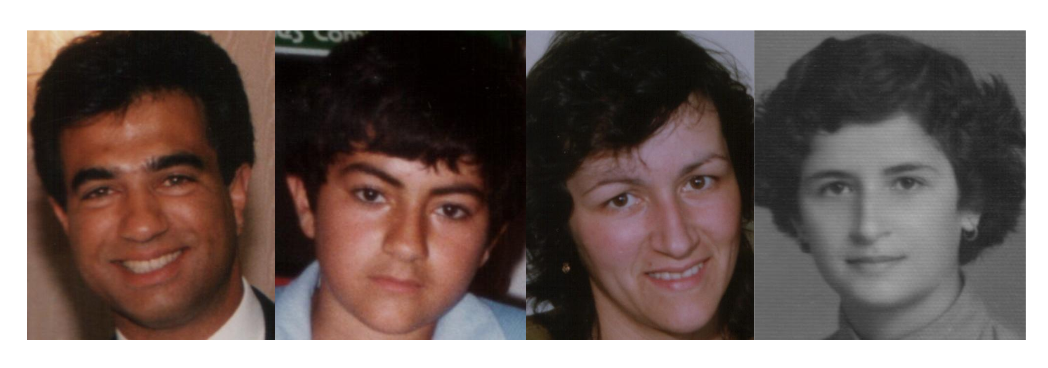
\includegraphics[width=\textwidth]{figures/FGNET_sample}
	\caption{FG-NET image samples.}
	\label{fig:imgSample1}
\end{figure}

\textbf{HuPBA-AgeGuess} dataset (\ref{fig:imgSample2}) used in this project is a subset of the 4865 images filtered out by a minimum number of votes per image. This subset contains 3398 face images. The images are captured in the wild so the faces position vary up to $\pm90º$ and the illumination is also different in every picture.

\begin{figure}[!h]
	\centering
	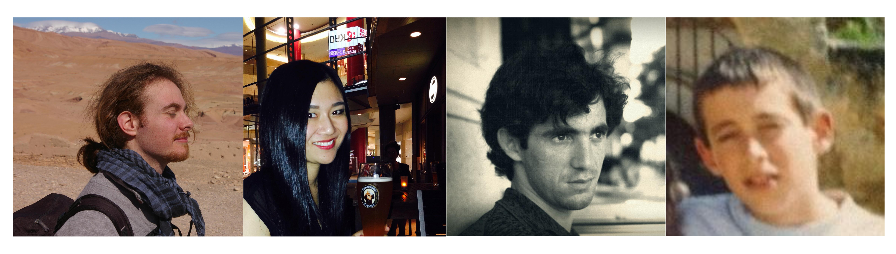
\includegraphics[width=\textwidth]{figures/HuPBA_sample}
	\caption{HuPBA-AgeGuess image samples.}
	\label{fig:imgSample2}
\end{figure}

Given the characteristics of the used descriptors in this work, both databases could be incremented by computing the mirror image, doubling the number of faces of each dataset (i.e. 2004 faces for the FG-NET and 6796 face images for the HuPBA-AgeGuess dataset).

\section{Evaluation Metrics} 

The two most commonly used evaluation metrics in age estimation are \acrfull{mae} and \gls{cs}.

The \gls{mae} is described as

\begin{equation}
MAE = \frac{1}{N}\sum_i^{N} |e_i|
\end{equation}

where $e_i$ is the error of the $ith$ instance, i.e. $e_i = |\hat{y_i} - y_i|$ where $y_i $ is the real label and $\hat{y_i}$ is the predicted label. This metric tells the average number of years that the prediction is wrong.

\gls{cs} is defined as the percentage of test images such that the absolute error is not higher than a threshold, $t$ (in years). i.e.,

\begin{equation}
CS(t) = (1 - \frac{1}{N}\sum_i^N h(|\hat{y_i} - y_i| - t))\cdot 100
\end{equation}
\begin{equation}
h(x) = 
\begin{cases}
1,				& \text{if } x \geq 0\\
0,              & \text{otherwise}
\end{cases}
\end{equation}

where $y_i$ is the age label of the $ith$ test image and $\hat{y_i}$ is the age prediction of the $ith$ test image.

\section{Experimental Settings}
This section describes the experimental setup and the parameters used in the two proposed methods.

\subsection{Biologically Inspired Method}

As described in Section \ref{sec:BIF} a \gls{svm} classifier and three \gls{svr} regressors were trained for this method. 

In order to find the best parameters a grid search was performed to find the best parameters. The parameters that formed the search space were the ones required by the \gls{svm} and \glspl{svr} and its kernels, which are the following:

\begin{itemize}
	\item \textbf{Penalty term ($C$)}: This is the Support Vector parameter that deals with the cost of a misclassification over all the classification task. 
	
	The $C$ parameters tried in the search space were between 0.1 and 2. The best parameters in the Age Group Classification were between 1 and 2 and the best parameters for the \glspl{svr} were between 0.1 and 1.
	
	\item \textbf{Influence term ($\gamma$)}: It is the \gls{rbf} kernel parameter. It determines how far the influence of a single training example reaches.
	
	The $\gamma$ parameters used were between 0.001 and 1, being between 0.001 and 0.01 the ones with better performance.
\end{itemize}

In order to train and validate the parameters a nested 10-fold cross validation technique was used.


\subsection{Deep Learning Method}

\section{Analysis of the Experiments}

\begin{figure}[!h]
	\centering
	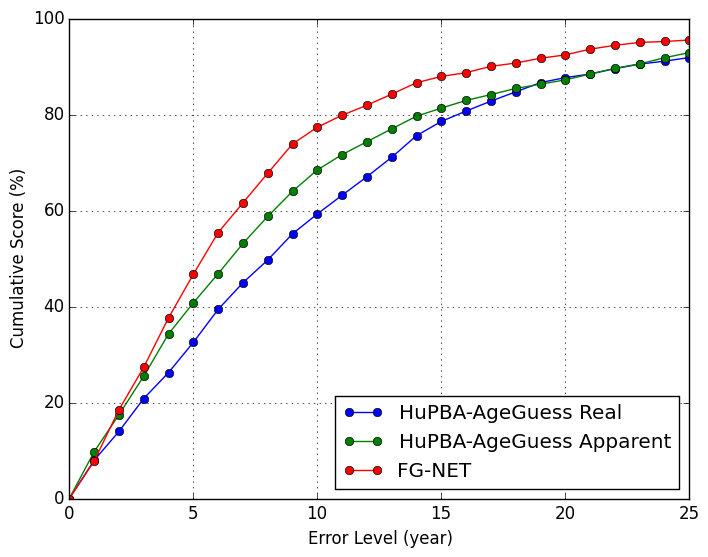
\includegraphics[width=\textwidth]{figures/cum_score}
	\caption{Cummulative Score }
	\label{fig:cumS}
\end{figure}

\chapter{Conclusions and Future work} \label{chap:conclusions}

\section{Conclusions}

\note{todo}

\section{Future Work}

\note{todo}

As a future work 

Analysis of the Challenge proposed methods.

Improve web-application

Increase database

Do face frontalization

% References
\renewcommand{\bibname}{\refname} % To change the heading of the chapter from Bibliography to References
\addcontentsline{toc}{chapter}{\bibname}
\bibliographystyle{plainnat}
%\nocite{*} % Should be removed at the end to make sure all references are cited
\bibliography{references}

\glsaddall
\printglossaries

\begin{appendices}
\chapter{Terms $\&$ Conditions}\label{cha:TaC}

The Terms and Conditions of the web-application are an adaptation to the ones of ChaLearn challenges\footnote{ChaLearn privacy policy: \url{http://www.chalearn.org/privacy.html}}. The general terms and conditions added to the ones described in ChaLearn are displayed below.

\begin{quote}
	\quote{
	\textit{The purpose of this Facebook application is to gather images of anonymous people labeled with an approximation of the estimated age. ChaLearn intends to use the data collected to organize a challenge in computer vision in which the participants will need to write programs that estimate a person’s age from a photo portrait.}
	
	\textit{By using this application you agree to:}
	
	\begin{itemize}
		\item \textit{Upload only images of photo portraits that you own or are authorized to use.}
		\item \textit{Grant ChaLearn the right to use these images in a public scientific competition and to conduct research in computer vision.}
		\item \textit{Not to upload images that are offending or illegal.}
	\end{itemize}
	}
\end{quote}
\end{appendices}

\end{document}


%1. Introduction
%  1.1. Motivation
%  1.2. Goals
%2. State of the art
%3. Resources
%  3.1. NAO and Wifibot
%  3.2. Kinect v2
%  3.3. ROS & SMACH
%  3.4. SOAR?
%4. The System
%  4.1. Architecture/Overview -> Diagramas, tipos de gestos
%  4.2. Computer Vision: Real Time OnLine Gesture Recognition
%            4.2.1. Dynamic Time Warping
%            4.2.2. Skeletal extracted features per gesture
%  4.3. Mobile Robotics: (Cognitive) Interaction
%            4.3.1. State Machines
%            4.3.2. Robot interaction (en este apartado 4.3 . no tengo muy claro como segmentarlo y que poner aún...)
%            4.3.3. Moving to a more general, cognitive approach (explicar cómo he jugado con SOAR y cómo se podria aplicar)
%5. Experimental evaluation
%            5.1 Data, methods, and settings
%            5.2 Gesture recognition evaluation
%            5.3 User experience evaluation (preguntas, experimento, y opiniones, todo junto)
%6. Conclusions and future work
%References